\documentclass[11pt,a4j]{jsarticle}
\title{光物性}
\author{1413176 三村幸祐}
\date{2016/10/26 \and 2016/11/02}
\usepackage{booktabs}
\usepackage[dvipdfmx,hiresbb]{graphicx}

\begin{document}
  
  
 \section{目的}
  ガラスや半導体などの対象に対して光の透過特性の測定を行うことで、その対象物の物性(半導体のバンドギャップ、ガラスの屈折率)を
  求める。
  
 \section{原理}
  \subsection{透過率$T$と反射率$R$}
   ある試料を強度$I_0$の光が透過する系を考える。
   
   透過率を$T$、反射率を$R$、透過光を$I_1$としたとき、入射面、出射面それぞれでも透過反射を考えて、
   \begin{eqnarray}
    I_1 &=& T I_0 = (1-R)^2 I_0 \\
    T &=& \frac{I_1}{I_0} = (1-R)^2 \\
    R &=& 1-\sqrt{T}
   \end{eqnarray}
   という関係が成り立つ。
   
   
  \subsection{ガラスと半導体の屈折率}
   まず、ガラスの屈折率は上記の反射率を用いて
   \begin{eqnarray}
   R &=& \frac{(n-1)^2}{(n+1)^2} \\
   n &=& \frac{1+\sqrt{R}}{1-\sqrt{R}} 
   \end{eqnarray}
   として求めることができる。
   
   屈折率を求めるにあたり、その波長による値のばらつきを見る指標にアッベ数というものがある。今回用いるC線(波長:656nm)、d線(588nm)、F線(486nm)により求めた屈折率をそれぞれ$n_C,n_d,n_F$とすると
   \begin{equation}
   アッベ数v_d = \frac{n_d - 1}{n_F - n_C}
   \end{equation}
   としてアッベ数は表され、この値が大きいほどばらつきが少ない、逆にこの値が小さいほどばらつきが多いことを示す。
   
   また、半導体の屈折率に関してはそれとは別に
   \begin{equation}
   n(\lambda) = 1.959 + \frac{0.257}{\lambda^2}
   \end{equation}
   という入射光の波長依存の独立した式により与えられる。
   
  \subsection{吸収と吸収係数}
   これまでは光の吸収がないとして考えてきたが、実際、特に今回の半導体などではどれだけ吸収されているのかが重要になってくる。
   その物質の吸収の度合いを測るための指標として、次によって与えられる光吸収係数$\alpha$が挙げられる。
   \begin{equation}
   \alpha = \frac{1}{L} ln(\frac{(1-R)^2}{T})
   \end{equation}
   ここで、$L$は半導体試料の厚さを表している。
   
   この光吸収係数と光子エネルギーの関係を表した値として、$\sqrt{\alpha h v}$が用いられる。
   横軸に光子エネルギー$hv$、縦軸に$\sqrt{\alpha h v}$をプロットしたグラフについて、
   励起過程(光子エネルギーに対して線形の領域)の直線を伸ばして横軸にぶつかった点の光子エネルギーは
   その半導体試料のエネルギーギャップに等しい。
   \begin{equation}
   \sqrt{\alpha hv} = B (hv - Eg)
   \end{equation}
   ($B$は任意定数)
   
  
  
 \section{測定手順}
  \subsection{実験1 ガラスの屈折率の測定}
	\begin{enumerate}
	\item C線(波長:656nm)、d線(588nm)、F線(486nm)について分光器を透過した光の強度($I_0$)を各波長3回ずつ測定。
	\item 上と同じ波長で顕微鏡用スライドガラスを入れた(透過させた)ときの透過光の光強度($I_1$)を各波長3回ずつ測定。
	\end{enumerate}
  
  \subsection{実験2 半導体試料(CdInGaS$_4$)の透過スペクトル、また吸収スペクトルによるエネルギーバンドギャップの測定}
  今回は私達のグループは厚み$L$が87$\mu m$のCdInGaS$_4$を使用した。
	\begin{enumerate}
	\item 分光器を透過した光の強度($I_0$)を400-700nmの波長域について適当な波長間隔で測定。
	\item 分光器出射口の試料ホルダーにCdInGaS$_4$をセットして、波長:500nm,600nm,700nmについて各3回ずつ透過強度を測定。再現性の確認に使用。
	\item サンプルを入れたまま、1と同様の操作をして光の透過強度($I_2$)を測定。
	\end{enumerate}
	
  \subsection{実験3 光ガラスフィルターの透過スペクトルの測定}
  各色の複数枚の光ガラスフィルターについて、それぞれの透過スペクトルの違いを測定して、フィルターとスペクトルの関係を考察。
   \begin{enumerate}
   \item 以下の光ガラスフィルターを用意。それぞれの透過光の測定する波長帯も以下の同表に示す。ここで光ガラスフィルターの型番は先頭のアルファベットが(Y:黄色、O:オレンジ、R:赤)、後半の2桁の数字がおよその透過波長(ex.)44:440nm,etc)を表している。
   \begin{table}[htb]
  \begin{center}
    \caption{使用する各光ガラスフィルターの色と測定波長帯}
    \begin{tabular}{ccccc} \toprule
光ガラスフィルター & 色 & 測定波長帯/nm \\ \midrule
Y44 & 薄黄 & 400~600 \\
Y52 & 黄 & 400 ~600 \\
O56 & オレンジ & 450~650 \\
R64 & 赤 & 550~750 \\ \bottomrule
    \end{tabular}
    \label{tab:price}
  \end{center}
\end{table}
  \item 上記の表を元に、各光ガラスフィルターを分光器の放射口に入れ、それぞれの光強度を測定。スペクトル分布を作成。
  \end{enumerate}
  
  
 \section{結果と考察}
  \subsection{実験1}
  
  スライドガラスについてF線、d線、C線の各波長での透過光と反射率の関係を表2に示めす。
  
  \begin{table}[htb]
  \begin{center}
    \caption{スライドガラスの各波長における透過光と反射率}
    \begin{tabular}{ccccc} \toprule
波長$\lambda$/nm & $I_0$/$\mu$W & $I_1$/$\mu$W & 反射率R \\ \midrule
486(F) & 1.55 & 1.38 & 0.0548 \\
588(d) & 2.87 & 2.64 & 0.0410 \\
656(C) & 2.49 & 2.30 & 0.0384 \\ \bottomrule
    \end{tabular}
    \label{tab:price}
  \end{center}
\end{table}

この実験結果より各波長におけるスライドガラスの屈折率、およびその平均は
  
  \begin{eqnarray}
  n_C &=& 1.49 \nonumber \\
  n_d &=& 1.51 \nonumber \\
  n_F &=& 1.61 \nonumber  \\
  n_{average} &=& 1.54 \nonumber 
  \end{eqnarray}
  となり、各値の平均値からの相対誤差は5%以内である。
  また式(6)よりアッベ数は
  \begin{equation}
  v_d = 4.08 \nonumber 
  \end{equation}
  となる。設計値からは理想のアッベ数値は60であるが、アッベ数を求める式(6)をみると分母でほぼ同じ大きさの$n_Fとn_C$の差をとっているため、その値は測定精度によって大きな桁落ちを起こしてしまう。たとえば、分子を0.5とすると、分母の差が0.01変わるだけでアッベ数は最大25減ってしまう。したがって、アッベ数を設計値の値として近づけるのは非常に困難と言える。
  
  \subsection{実験2}
  半導体試料の再現性の測定結果を次の表に示す。
  \begin{table}[htb]
  \begin{center}
    \caption{半導体の各波長での再現性(カッコ()内は、各波長の平均値からの誤差%)}
    \begin{tabular}{ccccc} \toprule
測定回数 & 500nm/nW & 600nm/nW & 700nm/nW \\ \midrule
1回目 & 294.7(0.569) & 1005(0) & 598.9(0.200) \\
2回目 & 294.3(0.432) & 1005(0) & 602.2(0.350) \\
3回目 & 290.1(1.00) & 1005(0) & 599.2(0.150) \\ \midrule
平均値 & 293.0 & 1005 & 600.1 \\ \bottomrule
    \end{tabular}
    \label{tab:price}
  \end{center}
\end{table}

  また、透過率Tを波長$\lambda$および光子エネルギー$hv$についてプロットしたグラフをそれぞれ図\ref{fig:T-lambda}と図\ref{fig:T-hv}に示した。
  \begin{figure}[htbp]
  \centering
  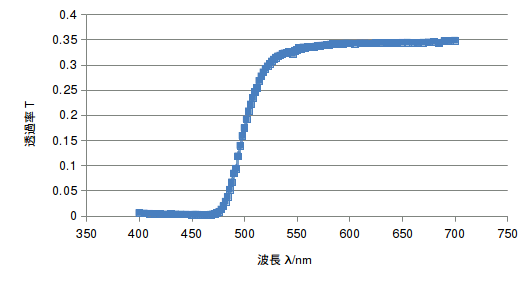
\includegraphics[width=8cm,clip]{1_2_T-lambda.png}
  \caption{半導体についての透過率Tと波長$\lambda$の関係}
  \label{fig:T-lambda}
 \end{figure}%
 
 \begin{figure}[htbp]
  \centering
  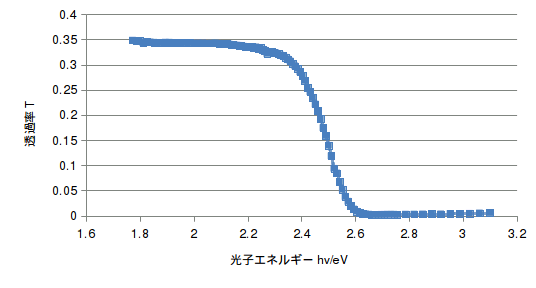
\includegraphics[width=8cm,clip]{1_2_T-hv.png}
  \caption{半導体についての透過率Tと光子エネルギー$hv$の関係}
  \label{fig:T-hv}
 \end{figure}%
 
 波長-透過率のグラフからは550nm以上の波長が透過しており、この波長は丁度可視光域の黄色のスペクトルと等しい。実際、目視で確認した所も半導体試料は黄色であった。
 
 また光子エネルギー-透過率のグラフも実質的には上のグラフと同じ情報しか乗っていないが、ここからはより吸収するエネルギーの関係が直感的に分かる。2.4eV以上のエネルギーを吸収していることからバンドギャップエネルギーが約2.4eV程度であることが予測できる。バンドギャップエネルギーについては後にも触れる。
  
  さらに次には光吸収係数の波長および光子エネルギーについての関係をそれぞれ図\ref{fig:alpha-lambda},\ref{fig:alpha-hv}に示す。
 
 \begin{figure}[htbp]
  \centering
  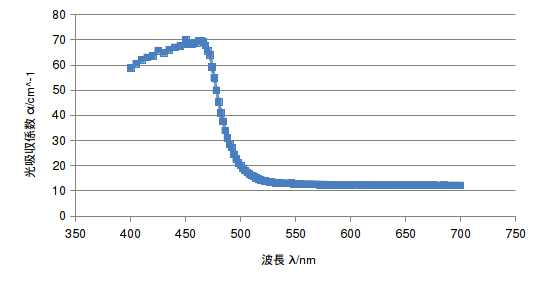
\includegraphics[width=8cm,clip]{1_2_alpha-lambda.png}
  \caption{半導体の光吸収係数$\alpha$-波長$\lambda$}
  \label{fig:alpha-lambda}
 \end{figure}%
 
 \begin{figure}[htbp]
  \centering
  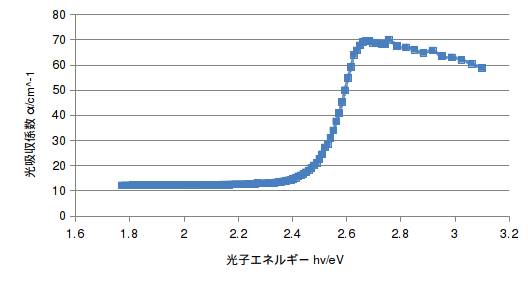
\includegraphics[width=8cm,clip]{1_2_alpha-hv.png}
  \caption{半導体の光吸収係数$\alpha$-光子エネルギー$hv$}
  \label{fig:alpha-hv}
 \end{figure}%
 
 この2つのグラフも先の透過率に関するグラフと同様な形式をとっている。ただし、こちらには透過波長域に傾きを持っていることが確認できる。これはバンドギャップと等しいエネルギーをもつ波長が最も吸収され、バンドギャップよりもエネルギーが大きくなるほどにバンドギャップに吸収されない余畳分が存在するためである。また反対のバンドギャップエネルギー以下の光子エネルギー領域で吸収係数が0になっていないことも分かる。これは低エネルギーの波長帯でも光の粒子性から、単位長さあたりでも一定の抵抗を生じて、熱エネルギーなどの形で損失してしまっているため、反射成分を除いて透過してくる光の損失分をすべて含んでしまう光吸収係数にも反映されてしまっているものと考える。これはこの半導体が間接遷移型半導体であることに起原をもつ。
 
 実験2の最後にはバンドギャップエネルギーを測定するために、光吸収係数の光子エネルギー依存性を図\ref{fig:alphahv-hv}に示す。
 
 \begin{figure}[htbp]
  \centering
  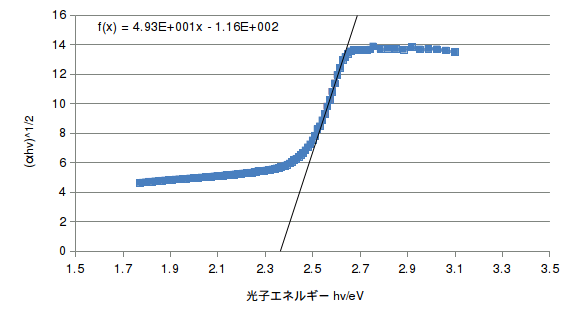
\includegraphics[width=8cm,clip]{1_2_alphahv-hv.png}
  \caption{半導体の光吸収係数$\alpha$の光子エネルギー$hv$依存性}
  \label{fig:alphahv-hv}
 \end{figure}%
 
 このグラフも今までと同様、グラフ中に吸収されていない領域、吸収され始める領域、完全にバンドギャップ分のエネルギーを吸収されている領域に、分けてみることができる。すると吸収されていく中程の領域は直線的に近似し、その線形関数は式(9)にしたがう。したがって式(9)からこの半導体のバンドギャップエネルギーは
 \begin{equation}
 E_g = 2.35eV \nonumber
 \end{equation}
 となる。文献値[1]と比較すると、
 \begin{eqnarray}
 E_g(文献値) &=& 2.38eV \nonumber \\
 実験値の文献値に対する相対誤差 &=& 1.34 % \nonumber
 \end{eqnarray}
 となる。約1%の誤差でバンドギャップエネルギーを求めることができたが、前期の透過率-光子エネルギーの関係グラフから予測した2.4eVも同等の誤差しか持たない。したがって透過率からも1,2%程度の精度でバンドギャップエネルギーを予測することができることもある。
  
  \clearpage
  
  \subsection{実験3}
  
  各色の光ガラスフィルターに関する透過率-波長の関係を図\ref{fig:Y44}から図\ref{fig:R64}に示す。
  
  \begin{figure}[htbp]
  \centering
  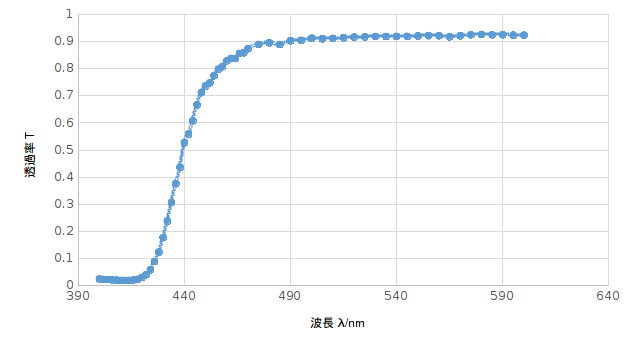
\includegraphics[width=8cm,clip]{2_3_Y44.png}
  \caption{Y44フィルターの透過率Tと波長$\lambda$の関係}
  \label{fig:Y44}
 \end{figure}%
  
  
  \begin{figure}[htbp]
  \centering
  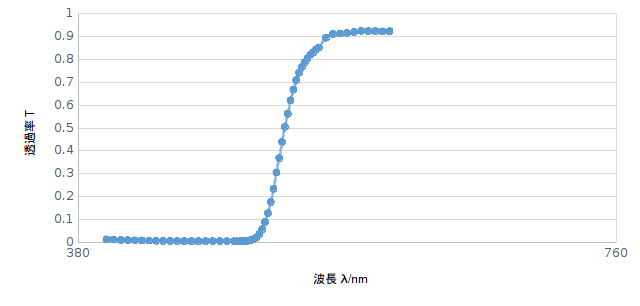
\includegraphics[width=8cm,clip]{2_3_Y52.png}
  \caption{Y52フィルターの透過率Tと波長$\lambda$の関係}
  \label{fig:Y52}
 \end{figure}%
 
 \begin{figure}[htbp]
  \centering
  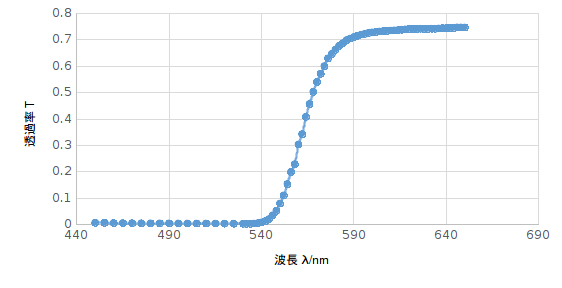
\includegraphics[width=8cm,clip]{2_3_O56.png}
  \caption{O56フィルターの透過率Tと波長$\lambda$の関係}
  \label{fig:56}
 \end{figure}%
 
 \begin{figure}[htbp]
  \centering
  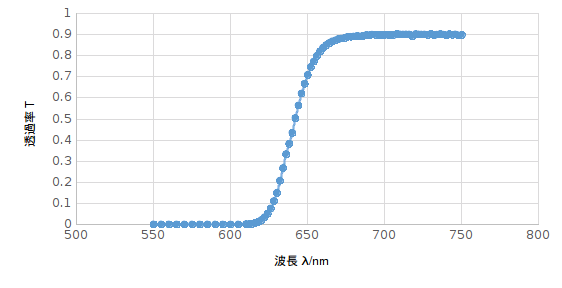
\includegraphics[width=8cm,clip]{2_3_R64.png}
  \caption{R64フィルターの透過率Tと波長$\lambda$の関係}
  \label{fig:R64}
 \end{figure}%
 
 この4つの色フィルターは同様に一定の波長を閾値としてそれ以上の波長を透過している。その閾値を見ていると、光フィルターの型番から、
 \begin{table}[htb]
  \begin{center}
    \caption{各色光ガラスフィルターの透過最小波長と設計値}
    \begin{tabular}{ccccc} \toprule
光フィルター & 透過最小波長/nm & 透過波長の設計値/nm \\ \midrule
Y44 & 460 & 440 \\
Y52 & 500 &520 \\
O56 & 560 & 560 \\
R64 & 650 & 640 \\ \bottomrule
    \end{tabular}
    \label{tab:price}
  \end{center}
\end{table}
として透過率が大きくなる閾値波長と、光フィルターの色に当たる波長が等しいことが確認できた。これはこの閾値波長相等のバンドギャップエネルギーをフィルターが持つため、それ以上のスペクトルを吸収してしまうためであろうと考える。
  
  \clearpage
  
 \section{実験課題}
  \begin{enumerate}
  \item 今回は各波長に対する入射光と出射光の強度の比から計算して吸収係数を求めたが、光が透過しきる前に(x$>$tで)十分に減衰してしまう場合、つまり
  \begin{eqnarray}
  exp(-\alpha t) &<& exp(-2) \nonumber \\
  -\alpha t &<& -2 \nonumber \\
  \alpha t &>& 2 \nonumber 
  \end{eqnarray}
  となる場合この方法は使用することができない。
  \item 光吸収係数がエネルギーバンドギャップ以下の光子エネルギー領域でもゼロにならなず、一定の値をとっている理由については「結果と考察」の「実験2」の項を参照。
  \item フィルターの色と透過率の関係については「結果と考察」の「実験3」の項を参照。
  \item 可視光の波長範囲は400nm(紫)から760(赤)である[2]。また色の見え方についてだが、網膜には画素ごとに赤、緑、青の各光に感度の高い3種の分光感度を持つ錐体がある。この3種の錐体の分光感度分布を$r(\lambda),g(\lambda),b(\lambda)$とし、スペクトル分布$E(\lambda)$を用いて脳への出力R,G,Bは
  \begin{eqnarray}
  R &=& \int E(\lambda) r(\lambda) d\lambda \nonumber \\
  G &=& \int E(\lambda) g(\lambda) d\lambda \nonumber \\
  B &=& \int E(\lambda) b(\lambda) d\lambda \nonumber
  \end{eqnarray}
  となる。このようにして、人間の目には、入射してきた光に関して上記の3色に感度をもち、各波長出力R,G,Bの組み合わせ(混色)によって、脳内で色を表現する[3]。
  \item 本実験を行うことで、物質による光の吸収の原理、透過反射の関係などを学ぶとともに、発展して色の仕組みについて考えるきっかけとなった。
  \end{enumerate}
  
  
 \section{参考文献}
  [1]T. IrieH. MiyashitaS. EndoH. Nakanishi, ''Photoluminescence of the layered compound CdInGaS4''(Study) 
  
  [2]国立天文台,''理科年表 平成28年度'',p.443 
  
  [3]長谷川伸,''画像工学'',コロナ社,p.31 
  

  


\end{document}